\documentclass[xetex,mathserif,serif,12pt]{beamer}

\usepackage[orientation=landscape,size=custom,width=16,height=9,scale=1]{beamerposter}

\usepackage{ifthen}
\usepackage{ifpdf}
\ifpdf
\usepackage{epstopdf}
\fi
\DeclareGraphicsExtensions{.mps,.eps,.png}

\usetheme{iywide}
\setbeamerfont{section in toc}{parent=structure,size=\small}
\setbeamerfont{subsection in toc}{parent=structure,size=\tiny}

\usepackage{hyperref}

\hypersetup{
  colorlinks,%
  citecolor=beamer@solarized@blue,%
  filecolor=beamer@solarized@blue,%
  linkcolor=beamer@solarized@blue,%
  urlcolor=beamer@solarized@blue%
}

\usepackage{fontspec}
\usepackage{xunicode}
\usepackage{xltxtra}
\setmainfont{Gill Sans}
\setmonofont[Scale=0.96]{Inconsolata}

\title{Cook like a Chef}
\author{Ian Yang}
\institute{Intridea Inc.}

\AtBeginSection[]
{
  \begin{frame}{Outline}
    \tableofcontents[currentsection]
  \end{frame}
}

\usepackage{bibentry}
\nobibliography*
\def\newblock{}

\usepackage{ctable}
\setlength{\heavyrulewidth}{0.1em}
\newcommand{\otoprule}{\midrule[\heavyrulewidth]}

\usepackage{textcomp}
\usepackage{listings}

\begin{document}

\lstset{
  language=Ruby,
  upquote=true,
  columns=fixed,
  numbers=left,
  numberstyle=\tiny\color{beamer@solarized@base01},
  numbersep=5pt,
  tabsize=2,
  extendedchars=true,
  breaklines=true,
  frame=single,
  showspaces=false,
  showtabs=false,
  xleftmargin=0pt,
  framexleftmargin=0pt,
  framexrightmargin=0pt,
  framextopmargin=0pt,
  framexbottommargin=0pt,
  showstringspaces=false,
  basicstyle=\footnotesize\ttfamily,
  keywordstyle=\color{beamer@solarized@green},
  stringstyle=\color{beamer@solarized@cyan}\ttfamily,
  identifierstyle=\color{beamer@solarized@blue},
  commentstyle=\color{beamer@solarized@base01},
  emphstyle=\color{beamer@solarized@red}
}

\begin{frame}
  \titlepage
\end{frame}

\section*{Contents}
\begin{frame}{Contents}
  \usebeamerfont{section in toc}
  \tableofcontents
\end{frame}

\section{What is Chef}
\label{sec:what}

\begin{frame}{What is Chef}
  \begin{itemize}
  \only<1>{\item a person who cooks professionally}
  \item<2-> an open-source \alert{system integration} framework that cooks your servers professionally
  \end{itemize}
\end{frame}

\begin{frame}
  \begin{figure}
    \centering
    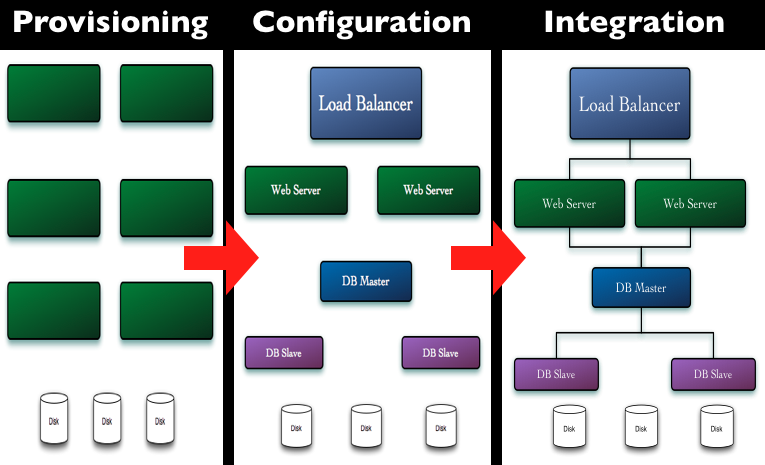
\includegraphics[height=6.5cm]{chefsi}
    \caption{\href{http://wiki.opscode.com/pages/viewpage.action?pageId=7274862}{What
        is Chef} from Chef Wiki}
    \label{fig:chefsi}
  \end{figure}
\end{frame}

\section{How Chef Works}
\label{sec:how-work}

\begin{frame}
  \begin{figure}
    \centering
    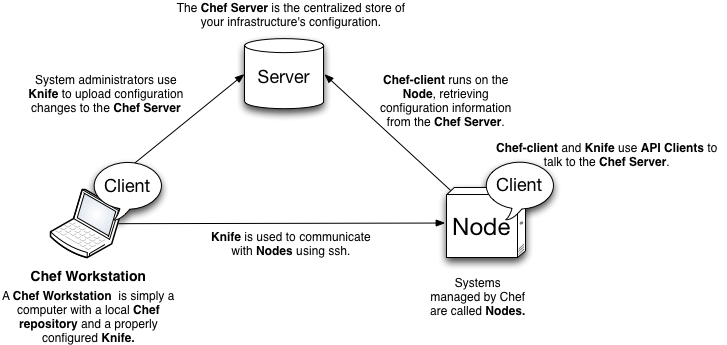
\includegraphics[height=5.8cm]{chef-basics-nwc}
    \caption{\href{http://wiki.opscode.com/display/chef/Architecture+Introduction}{Arch Intro} from Chef Wiki}
    \label{fig:chefsi}
  \end{figure}
\end{frame}

\begin{frame}{Components}
  \begin{description}[<+->]
  \item[chef] Gem of client/solo run-time and CLI tools.
  \item[chef-server] Gem of server run-time
  \item[Chef Repo] \href{https://github.com/opscode/chef-repo}{Blank repo template}
  \item[Community] \href{http://community.opscode.com/}{Cookbooks hosting site}
  \end{description}
\end{frame}

\begin{frame}{Solo Workflow}
  \begin{enumerate}[<+->]
  \item Collect \alert{Node} info (\alert{ohai})
  \item Get \alert{Node} configuration data
  \item Run specified \alert{Recipes} with \alert{Node} info and configuration data
  \end{enumerate}
\end{frame}

\begin{frame}{Recipes}
  \begin{description}[<+->]
  \item[Recipes] configuration steps by \alert{Resources}
  \item[Resources] cross platform abstraction of tasks
  \item[Providers] actually execute the Resources
  \end{description}
\end{frame}

\begin{frame}[fragile]
  \frametitle{Git Recipe}
  \begin{beamer@nomargin}
  \begin{lstlisting}
case node[:platform] # node info
when "debian", "ubuntu"
  package "git-core" # package is a resource
else 
  package "git"
end
  \end{lstlisting}  
  \end{beamer@nomargin}
\end{frame}

\section{How to Use Chef}
\label{sec:how-use}

\section{Real Examples}
\label{sec:ex}
 
\end{document}
